%%%---%%%---%%%---%%%---%%%---%%%---%%%---%%%---%%%---%%%---%%%---%%%---%%%---%%%---%%%---%%%---%%%---%%%---%%%---%%%---%%%---%%%---%%%---%%%---%%%
%
\chapter{Overview of the solution}
%
%%%---%%%---%%%---%%%---%%%---%%%---%%%---%%%---%%%---%%%---%%%---%%%---%%%---%%%---%%%---%%%---%%%---%%%---%%%---%%%---%%%---%%%---%%%---%%%---%%%
This chapter presents the main functionality of the debugging tool in all generalities and presents how it has been integrated with Intellij IDE as a GUI plugin.

\section{side note}

	\begin{itemize}
		\item at first : we wanted to work on top of the IDE debugger
		\item but from plugin it is difficult to access the implementation for the debugger
		\item made me think about what is important for debugging grammar ?
		\item important thing is to be able to see the execution trace of the parsers
		\item being able to look at the parse state the system was in when the parser was called
		\item to be able to see the portion of the input matched by the parser
		\item it is possible to access all this information without stopping the execution
		\item the syntax tree generated by the parse can by analyze and we can simulate time traveling in the parse execution
	\end{itemize}
% Discuss that having a debugger is one good thing, but as is, it is not very useful, we need a tool to harness its power. Explain that we build
% this plugin as a tool for the final user to use and develop his own parsers and grammar. This part has been created with the users need in mind
% to be as friendly user as possible.
	%%%---%%%---%%%---%%%---%%%---%%%---%%%---%%%---%%%---%%%---%%%---%%%---%%%---%%%---%%%---%%%---%%%---%%%---%%%---%%%---%%%---%%%---%%%---%%%---%%%
	\section{Overview of the fonctionality}

	%%%---%%%---%%%---%%%---%%%---%%%---%%%---%%%---%%%---%%%---%%%---%%%---%%%---%%%---%%%---%%%---%%%---%%%---%%%---%%%---%%%---%%%---%%%---%%%---%%%
	At this point we know the context, we know autumn and we know the motivations. From here we don't discuss why but how.

	\begin{itemize}
		\item Autumn implementation of parser as function -> changed into objects to create hooks for debugger.
		\item neet to rewrite java grammar to reflect changes in the parsers implementation
		\item debugger is a function that is hooked on the execution of each parsers
		\item during execution a syntax tree is build
		\item each node of the syntax tree contains informations about the parse state at the moment of the parser invocation
		\item those information can then be processed and displayed on a GUI for the developper to reason about
		\item ULM chart of the debugger and how it connects to autumn
	\end{itemize}



	% We developped a debugger, to do so we had to adapt autumn parsers. Parsers were initially boolean functions, we transformed them into objects that can be manipulated and stored to remember which parsers were called and in which order during runtime
	\begin{itemize}
		\item debuging tool = hook on top of parser's definition
		\item builds up a syntax tree
		\item which is then read and displayed by a GUI
		\item the GUI is implemented as a IDE plugin
	\end{itemize}

	\subsection{Intellij plugin}

	\begin{itemize}
		\item intellij plugin is essentially a panel that can be docked on top of the IDE
		\item it presents the data in several different forms
		\item the data can then be filtered to pinpoint specific problems
	\end{itemize}

	\begin{figure}[h]
		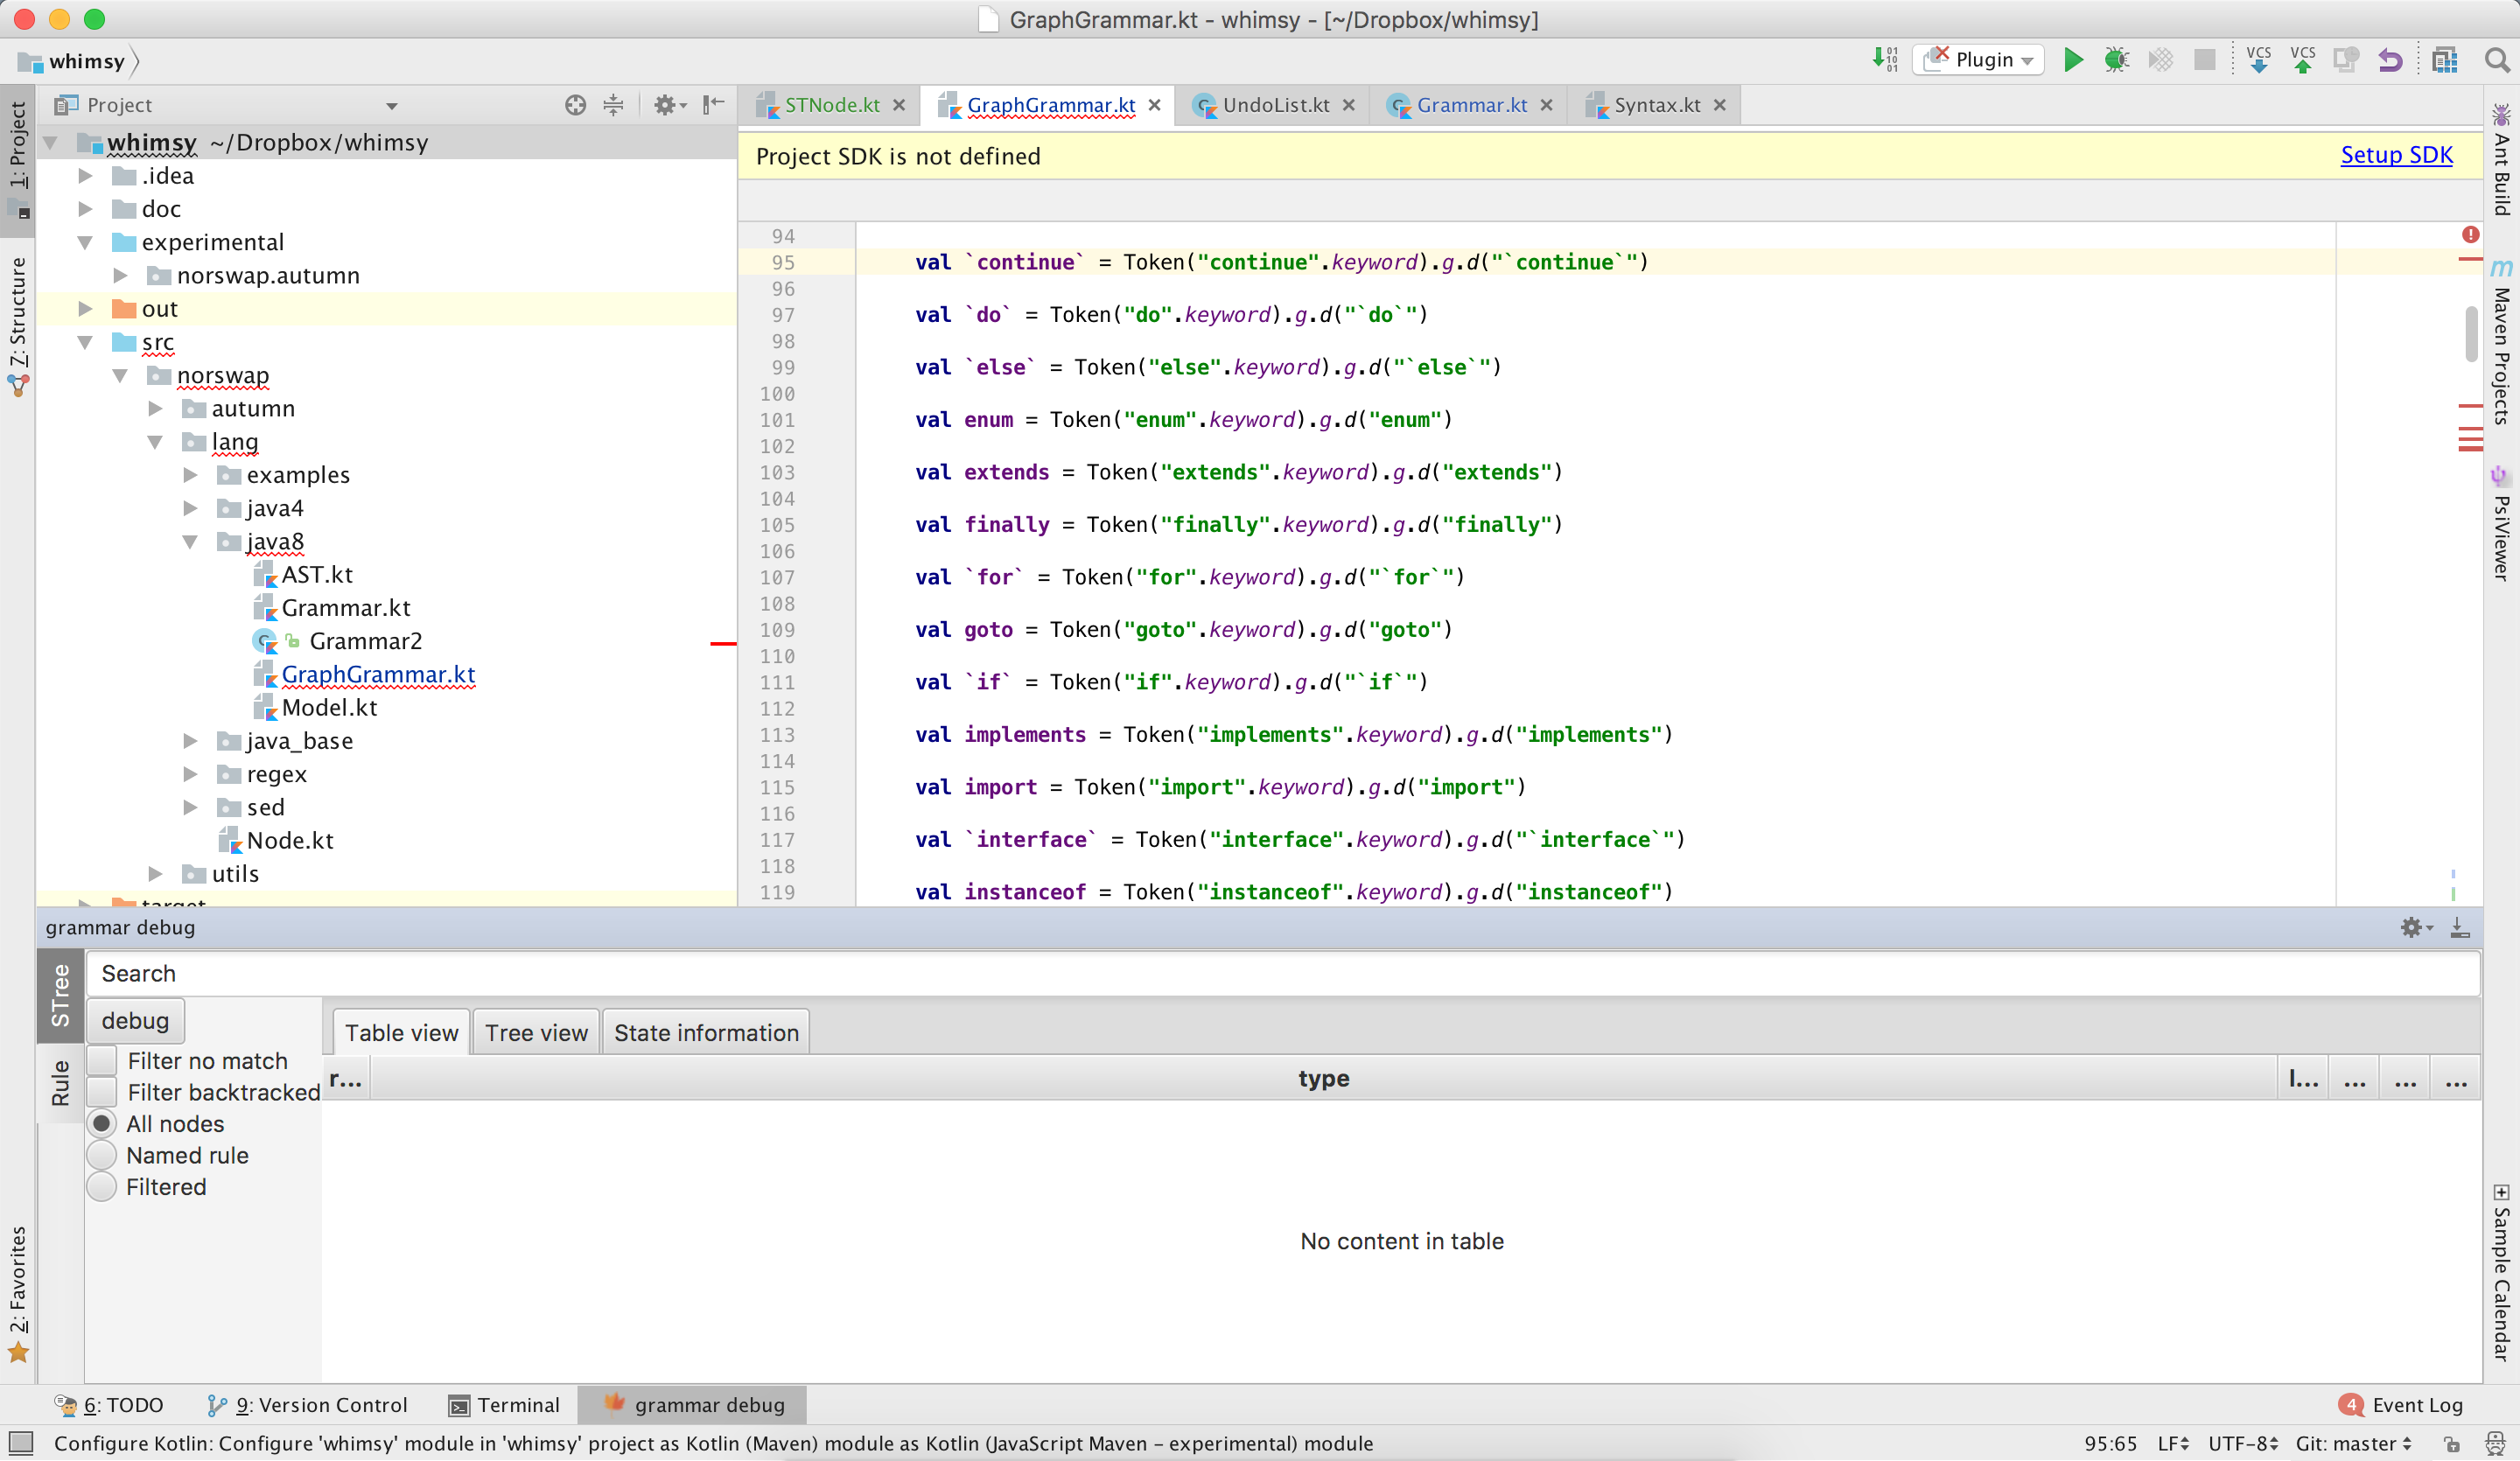
\includegraphics[width=1\textwidth] {ressources/intj_plug}
		\caption{IDE GUI for Autumn's debuggin tool} 
		\label{fig:intj_plug}
	\end{figure}

		% \paragraph{The debugger} works a posteriori, that means that it attempt to parser the file using the provided grammar and then display useful information about the parse. At first, the way we invision the debugger was more in the line of what general purpose debuggers do, executing the code and stopping at breakpoints, allowing the user to step into, over or resume the execution of the code. We wanted our debugger to work as a layer on top of Intellij's general purpose debugger. However, the difficulties of working with Intellij's debugger for the developpement of a plugin lead us to rething our solution.

		% We tried to get in the shoes of the grammar developper, while trying to troubleshoot his work, what does he really need to know ? The most important information for him is to be able to see which rule of the grammar has matched with what part of the input, and to be able to follow the sequence of parser calls. All those information are available almost for free. Throughout its execution, Autumn maintain a log of modification of the state, it is therefore possible to retrace the execution of the parsers using the syntax tree and regenerating the state corresponding to the call of a specific parser. So in practice, we eliminated the need to stop the execution at one point since we can display the execution trace and regenerate the state in which the parser was during the call, effectively providing the user with the tools needed to analyze the execution of the parser and similating the step in, over and backward a general purpose debugger would have.


		\begin{figure}[h]
			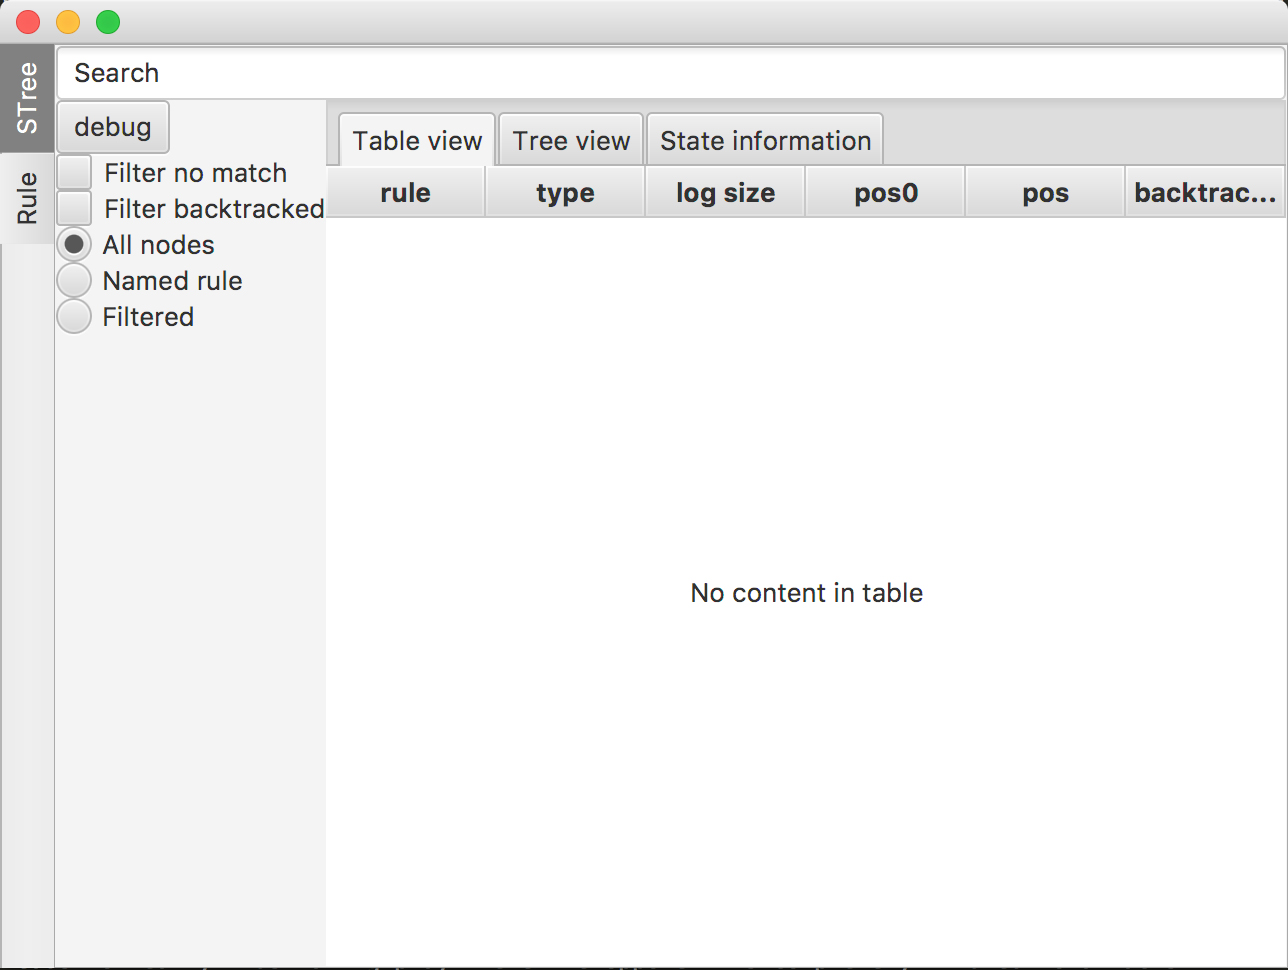
\includegraphics[width=1\textwidth] {ressources/stand_alone}
			\caption{Stand alone view - the debugger GUI can be executed independetly from the IDE albeit some restrictions} 
			\label{fig:stand_alone}
		\end{figure}


		\begin{figure}[h]
			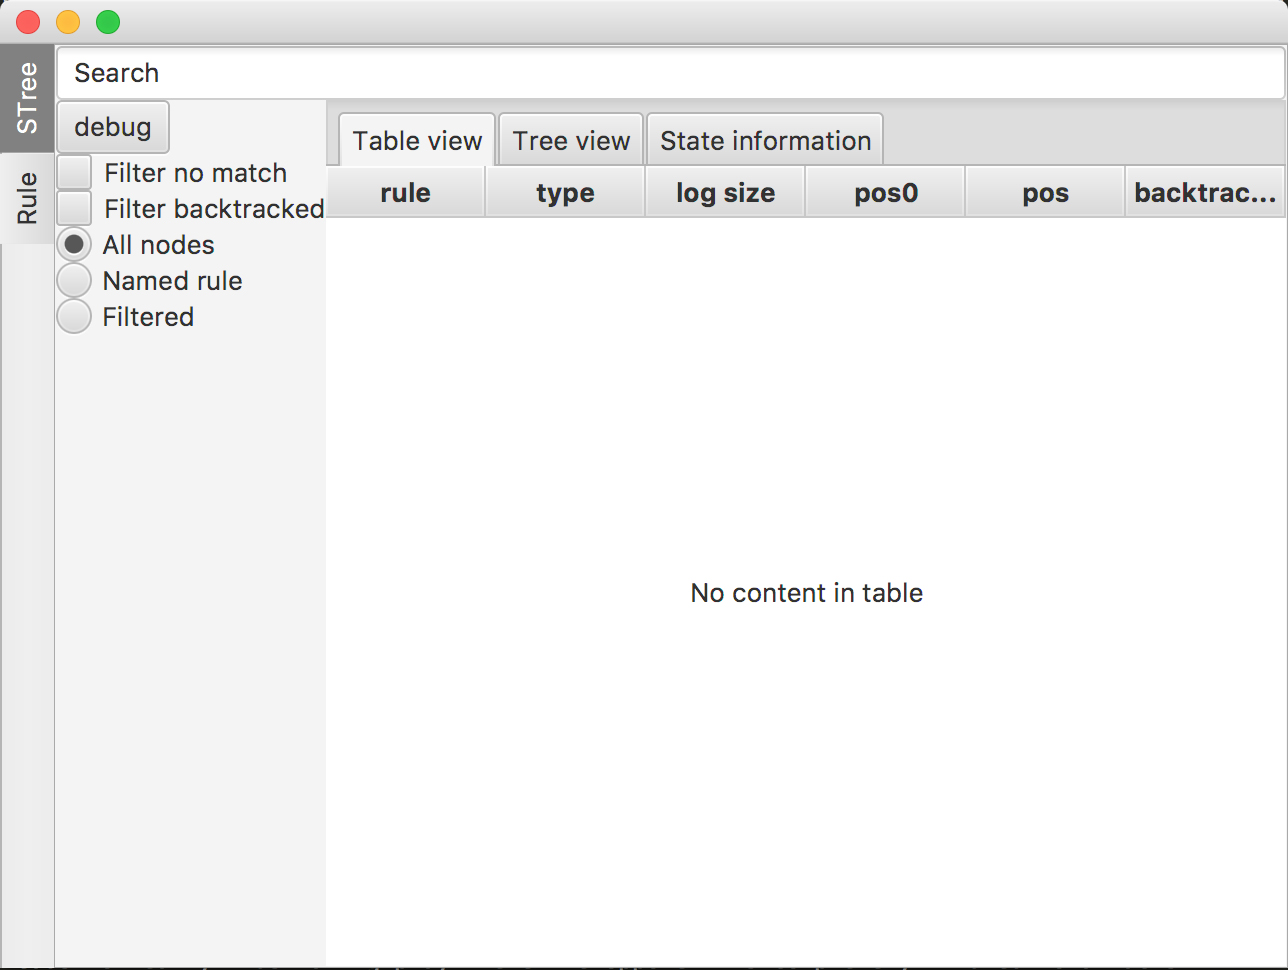
\includegraphics[width=1\textwidth] {ressources/stand_alone}
			% \caption{Stand alone view - the debugger GUI can be executed independetly from the IDE albeit some restrictions} 
			% \label{fig:stand_alone_detailed}
		\end{figure}


		%%%---%%%---%%%---%%%---%%%---%%%---%%%---%%%---%%%---%%%---%%%---%%%---%%%---%%%---%%%---%%%---%%%---%%%---%%%---%%%---%%%---%%%---%%%---%%%---%%%
		\subsection{Views}
		%%%---%%%---%%%---%%%---%%%---%%%---%%%---%%%---%%%---%%%---%%%---%%%---%%%---%%%---%%%---%%%---%%%---%%%---%%%---%%%---%%%---%%%---%%%---%%%---%%%
		\paragraph{Table view - Execution trace} The table view highlight the execution sequence of the parsers

		\begin{itemize}
			\item execution trace
			\item allow to see the sequence of parsers that were called chronologically
		\end{itemize}

		\begin{figure}[h]
			\centering
			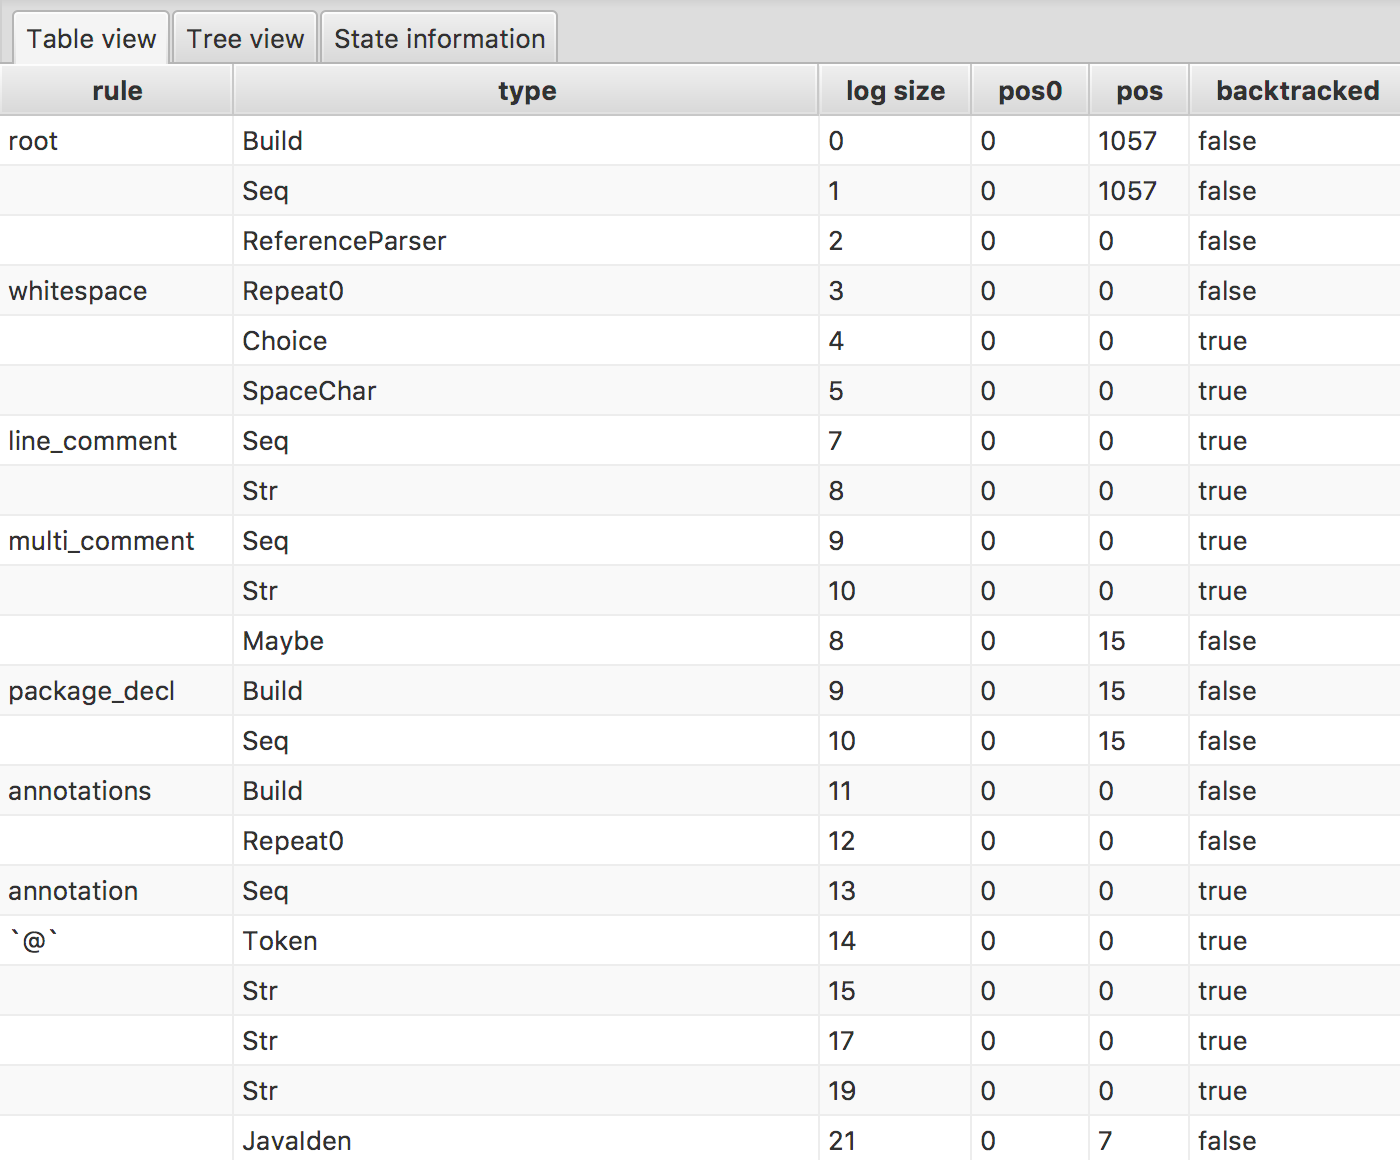
\includegraphics[width=.7\textwidth] {ressources/tableview}
			\caption{} 
			\label{fig:tableview}
		\end{figure}
		\paragraph{Tree view - Syntax tree} The tree view highlight the hierarchy of the parsers

		\begin{itemize}
			\item highlight the hierarchy between parsers and rules
		\end{itemize}

		\begin{figure}[h]
			\centering
			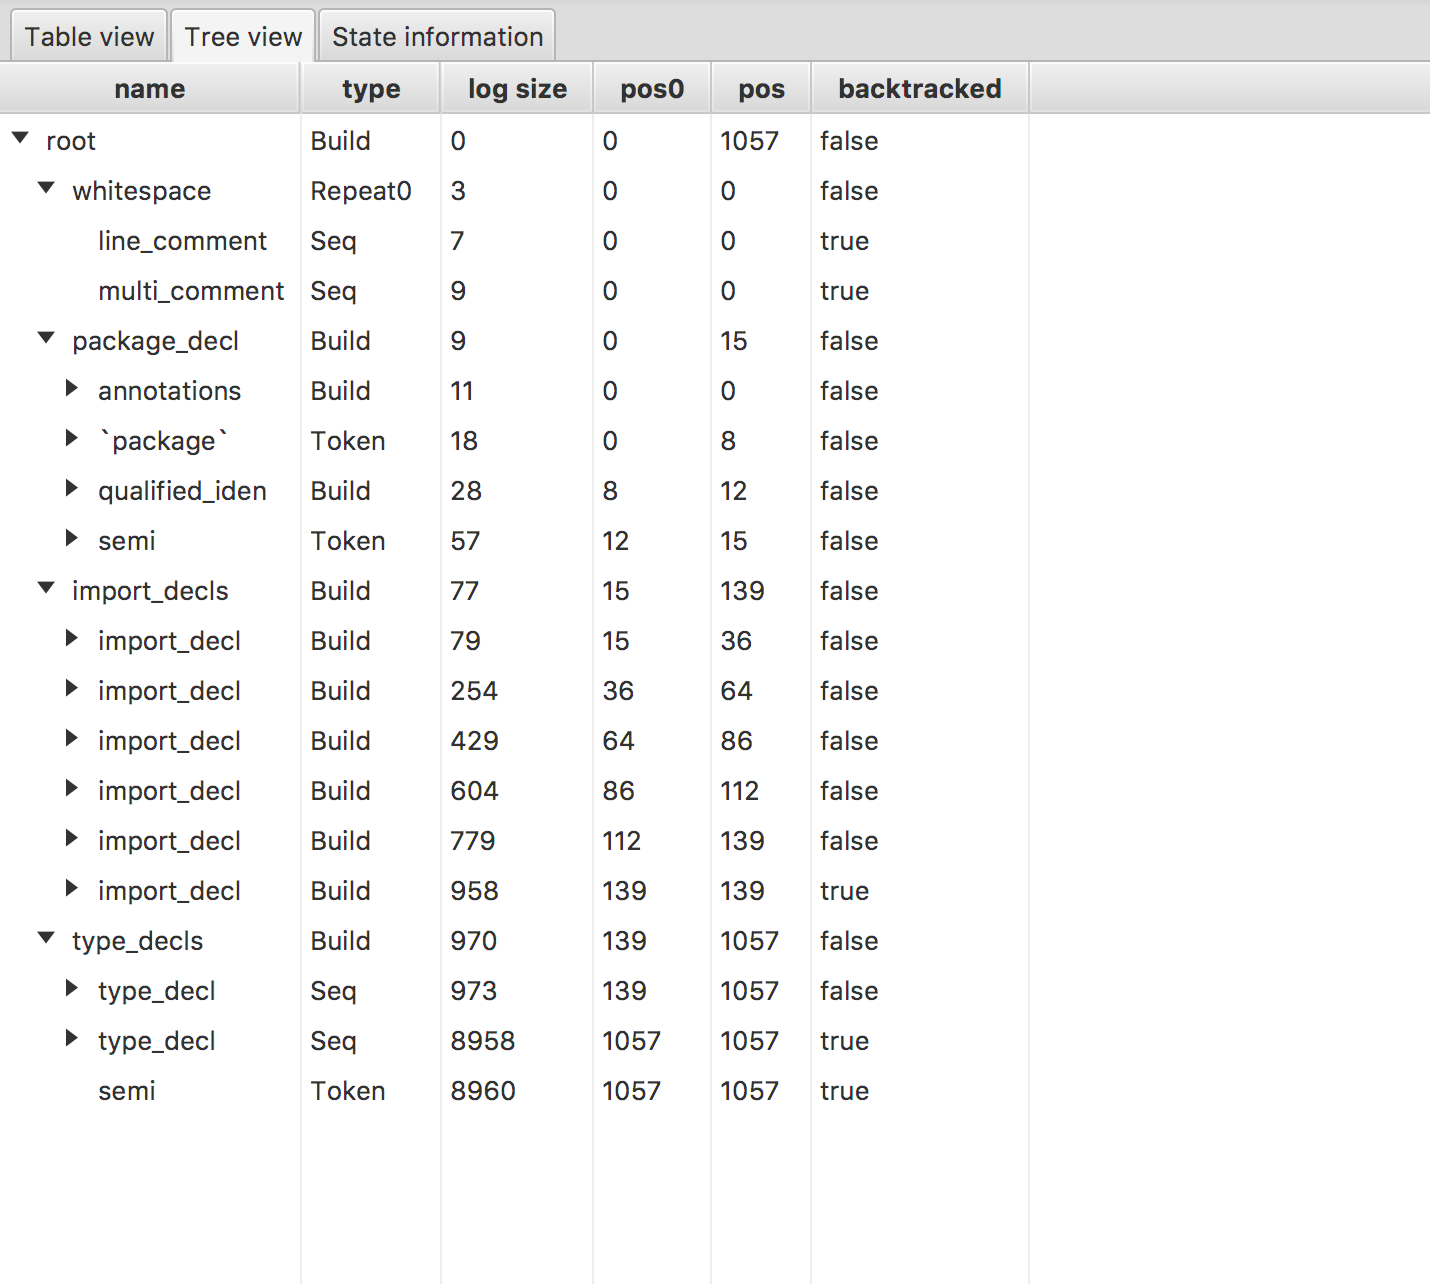
\includegraphics[width=.7\textwidth] {ressources/treeview}
			\caption{} 
			\label{fig:treeview}
		\end{figure}

		\paragraph{State information} This tab display the current state


		%%%---%%%---%%%---%%%---%%%---%%%---%%%---%%%---%%%---%%%---%%%---%%%---%%%---%%%---%%%---%%%---%%%---%%%---%%%---%%%---%%%---%%%---%%%---%%%---%%%
		\subsection{Filtering the informations}
		%%%---%%%---%%%---%%%---%%%---%%%---%%%---%%%---%%%---%%%---%%%---%%%---%%%---%%%---%%%---%%%---%%%---%%%---%%%---%%%---%%%---%%%---%%%---%%%---%%%

		\begin{itemize}
			\item all this information is overwhelming and not very usefull (like a dump of info)
			\item filter allow to select the relevant informations the user might be reasoning with
			\item filter possibilities
			\item unamed: unamed parser which doesn't match the rule one to one 
			\item backtracked
			\item no match : nodes that didn't match anything in the input but succeded
		\end{itemize}

		% Because we don't stop the execution with breakpoints, the user will get the entire execution trace and all the related information with it at once. This can be a little bit overwhelming and therefore defeat the purpose of the debugger. To facilitate the navigation of thoses information we create filtering tools. The user can decide what to display at anytime. The different filters fill in different roles. It is possible to filter the unamed parser which doesn't match the rule one to one to get a ``higher'' level view of the parsing. One can filter out the node that backtracked to see exactly how the input has been matched. Because of the nature of certain parsers, there will be nodes that didn't match anything in the input but succeded anyway and therefore didn't backtracked, those nodes are filterable as well. And finally, because the user might be interested only in the matching of a particular rule or parser, there is a search field in which we can input the name of the parser of interest to filter everything else out.
